% --- Page Style ---
\pagestyle{fancy}
\fancyhf{}
\lhead{Algebra --- Unit 1}
\rhead{Exam ID: \underline{\hspace{2cm}}}
\lfoot{Show all work. No calculators.}
\rfoot{Page \thepage}
\renewcommand{\headrulewidth}{0.4pt}
\renewcommand{\footrulewidth}{0.4pt}

% --- Header spanning both columns ---
\twocolumn[
  \begin{center}
    {\huge \textbf{Unit 1 Test}} \\
    \vgap
    {\large \textbf{Algebra}} \\
    \vgap
    \begin{tabular}{|l|l|}
      \hline
      \textbf{Student Name:} & \hspace{6cm} \\ \hline
      \textbf{Date:} & \hspace{6cm} \\ \hline
    \end{tabular}
  \end{center}
  \vgap
  \textbf{Instructions:} Show all work as necessary. No calculators are allowed for this assessment.
  \vgap
]

% % --- Form A (Questions 1--5) ---
% \section*{Form A}

% \begin{enumerate}[leftmargin=*, label=\textbf{\arabic*.}]

%   \item Simplify: $\sqrt[3]{200}(\sqrt[3]{135}+\sqrt[3]{40})$. \points{2}
%   \vgappp

%   \item Graph $g(x)=2\sqrt{6-x}-1$ on the axes below and use it to find the key features requested. Remember to clearly include at least 3 points on the graph of $g(x)$. \points{8}

%   \begin{center}
%   \begin{tikzpicture}[x=0.35cm, y=0.35cm, line cap=round, line join=round]
%     \draw[thick,->] (-2,0) -- (8,0) node[right] {$x$};
%     \draw[thick,->] (0,-2) -- (0,6) node[above] {$y$};
%     \foreach \x in {-2,0,2,4,6,8} \draw (\x,2pt) -- (\x,-2pt) node[below,font=\scriptsize] {\x};
%     \foreach \y in {-2,0,2,4,6} \draw (2pt,\y) -- (-2pt,\y) node[left,font=\scriptsize] {\y};
%     \draw[gray!40] (-2,-2) grid[step=1] (8,6);
%   \end{tikzpicture}
%   \end{center}

%   Domain: \blank[4em]

%   Range: \blank[4em]

%   Interval(s) of Increase: \blank[4em]

%   Interval(s) of Decrease: \blank[4em]

%   Concave Up: \blank[4em]

%   Concave Down: \blank[4em]
%   \vgapp

%   \item Which of the following BEST describes the behavior of $g(x)$ over the interval $[-27,-9]$? \points{1}

%   \begin{tasks}(1)
%     \task Increasing with a decreasing rate of change
%     \task Decreasing with an increasing rate of change
%     \task Increasing with an increasing rate of change
%     \task Decreasing with a decreasing rate of change
%   \end{tasks}
%   \vgap

%   \item Solve the equation for $x$. Express all algebraic solutions. Then indicate any extraneous solutions. If there are no extraneous solutions, write ``no extraneous solutions.'' \points{4}
%   \[
%   x - 2 = -2\sqrt{x-3}
%   \]
%   \vgappp

%   \item Finish graphing $f(x)$ on the axes provided below. Then, identify the key features requested. All intervals MUST be expressed in interval notation (including concave up and concave down). \points{12}
%   \[
%   f(x)= \begin{cases}
%     -(x+3)^{2}+4 & -6 \leq x<-2 \\
%     1-x & -2<x<0 \\
%     \sqrt{1+x}+2 & 0 \leq x<3 \\
%     \dfrac{x+7}{2} & 3<x \leq 5
%   \end{cases}
%   \]

%   \begin{center}
%   \begin{tikzpicture}[x=0.28cm, y=0.28cm, line cap=round, line join=round]
%     \draw[thick,->] (-7,0) -- (6,0) node[right] {$x$};
%     \draw[thick,->] (0,-3) -- (0,7) node[above] {$y$};
%     \foreach \x in {-6,-4,-2,0,2,4,6} \draw (\x,2pt) -- (\x,-2pt) node[below,font=\scriptsize] {\x};
%     \foreach \y in {-2,0,2,4,6} \draw (2pt,\y) -- (-2pt,\y) node[left,font=\scriptsize] {\y};
%     \draw[gray!40] (-7,-3) grid[step=1] (6,7);
%   \end{tikzpicture}
%   \end{center}

%   Domain: \blank

%   Range: \blank

%   Interval(s) of Increase: \blank

%   Interval(s) of Decrease: \blank

%   Concave Up: \blank

%   Concave Down: \blank

%   Absolute Minimum: \blank

%   Absolute Maximum: \blank

%   $\displaystyle \lim_{x \to 0^{-}} f(x) = $ \blank
%   \vgapp

% \end{enumerate}

% \clearpage
% % --- Form B (Questions 6--10) ---
% \section*{Form B}

% \begin{enumerate}[leftmargin=*, label=\textbf{\arabic*.}, resume]

%   \item Simplify: $2\sqrt[3]{32}(\sqrt[3]{16}-\sqrt[3]{54})$. \points{2}
%   \vgappp

%   \item Graph $g(x)=-2\sqrt{7-x}+2$ on the axes below and use it to find the key features requested. Remember to clearly include at least 3 points on the graph of $g(x)$. \points{8}

%   \begin{center}
%   \begin{tikzpicture}[x=0.35cm, y=0.35cm, line cap=round, line join=round]
%     \draw[thick,->] (-2,0) -- (8,0) node[right] {$x$};
%     \draw[thick,->] (0,-2) -- (0,6) node[above] {$y$};
%     \foreach \x in {-2,0,2,4,6,8} \draw (\x,2pt) -- (\x,-2pt) node[below,font=\scriptsize] {\x};
%     \foreach \y in {-2,0,2,4,6} \draw (2pt,\y) -- (-2pt,\y) node[left,font=\scriptsize] {\y};
%     \draw[gray!40] (-2,-2) grid[step=1] (8,6);
%   \end{tikzpicture}
%   \end{center}

%   Domain: \blank[4em]

%   Range: \blank[4em]

%   Interval(s) of Increase: \blank[4em]

%   Interval(s) of Decrease: \blank[4em]

%   Concave Up: \blank[4em]

%   Concave Down: \blank[4em]
%   \vgapp

%   \item Which of the following BEST describes the behavior of $g(x)$ over the interval $[-9,-3]$? \points{1}

%   \begin{tasks}(1)
%     \task Increasing with a decreasing rate of change
%     \task Decreasing with an increasing rate of change
%     \task Increasing with an increasing rate of change
%     \task Decreasing with a decreasing rate of change
%   \end{tasks}
%   \vgap

%   \newpage
%   \item Solve the equation for $x$. Express all algebraic solutions. Then indicate any extraneous solutions. If there are no extraneous solutions, write ``no extraneous solutions.'' \points{4}
%   \[
%   2 - x = -2\sqrt{5-x}
%   \]
%   \vgappp

%   \item Finish graphing $f(x)$ on the axes provided below. Then, identify the key features requested. All intervals MUST be expressed in interval notation (including concave up and concave down). \points{12}
%   \[
%   f(x)= \begin{cases}
%     (x+3)^{2}+2 & -5 \leq x<-2 \\
%     1-x & -2<x<0 \\
%     -\sqrt{1+x}-2 & 0 \leq x<3 \\
%     \dfrac{x-5}{2} & 3<x \leq 5
%   \end{cases}
%   \]

%   \begin{center}
%   \begin{tikzpicture}[x=0.28cm, y=0.28cm, line cap=round, line join=round]
%     \draw[thick,->] (-7,0) -- (6,0) node[right] {$x$};
%     \draw[thick,->] (0,-4) -- (0,7) node[above] {$y$};
%     \foreach \x in {-6,-4,-2,0,2,4,6} \draw (\x,2pt) -- (\x,-2pt) node[below,font=\scriptsize] {\x};
%     \foreach \y in {-2,0,2,4,6} \draw (2pt,\y) -- (-2pt,\y) node[left,font=\scriptsize] {\y};
%     \draw[gray!40] (-7,-4) grid[step=1] (6,7);
%   \end{tikzpicture}
%   \end{center}

%   Domain: \blank

%   Range: \blank

%   Interval(s) of Increase: \blank

%   Interval(s) of Decrease: \blank

%   Concave Up: \blank

%   Concave Down: \blank

%   Absolute Minimum: \blank

%   Absolute Maximum: \blank

%   $\displaystyle \lim_{x \to 3^{-}} f(x) = $ \blank
%   \vgapp

% \end{enumerate}

% \clearpage
% % --- Form C (Questions 11--15) ---
% \section*{Form C}

% \begin{enumerate}[leftmargin=*, label=\textbf{\arabic*.}, resume]

%   \item Simplify: $2\sqrt[3]{250}(\sqrt[3]{32}-\sqrt[3]{108})$. \points{2}
%   \vgappp

%   \item Graph $g(x)=2\sqrt{4-x}-2$ on the axes below and use it to find the key features requested. Remember to clearly include at least 3 points on the graph of $g(x)$. \points{8}

%   \begin{center}
%   \begin{tikzpicture}[x=0.35cm, y=0.35cm, line cap=round, line join=round]
%     \draw[thick,->] (-2,0) -- (8,0) node[right] {$x$};
%     \draw[thick,->] (0,-3) -- (0,6) node[above] {$y$};
%     \foreach \x in {-2,0,2,4,6,8} \draw (\x,2pt) -- (\x,-2pt) node[below,font=\scriptsize] {\x};
%     \foreach \y in {-2,0,2,4,6} \draw (2pt,\y) -- (-2pt,\y) node[left,font=\scriptsize] {\y};
%     \draw[gray!40] (-2,-3) grid[step=1] (8,6);
%   \end{tikzpicture}
%   \end{center}

%   Domain: \blank[4em]

%   Range: \blank[4em]

%   Interval(s) of Increase: \blank[4em]

%   Interval(s) of Decrease: \blank[4em]

%   Concave Up: \blank[4em]

%   Concave Down: \blank[4em]
%   \vgapp

%   \item Which of the following BEST describes the behavior of $g(x)$ over the interval $[-19,-9]$? \points{1}

%   \begin{tasks}(1)
%     \task Increasing with a decreasing rate of change
%     \task Decreasing with an increasing rate of change
%     \task Increasing with an increasing rate of change
%     \task Decreasing with a decreasing rate of change
%   \end{tasks}
%   \vgap

%   \newpage
%   \item Solve the equation for $x$. Express all algebraic solutions. Then indicate any extraneous solutions. If there are no extraneous solutions, write ``no extraneous solutions.'' \points{4}
%   \[
%   3 - x = -2\sqrt{x-3}
%   \]
%   \vgappp

%   \item Finish graphing $f(x)$ on the axes provided below. Then, identify the key features requested. All intervals MUST be expressed in interval notation (including concave up and concave down). \points{12}
%   \[
%   f(x)= \begin{cases}
%     (x+3)^{2}-2 & -4<x \leq -1 \\
%     -x+4 & -1<x<1 \\
%     -\sqrt{x-1}-2 & 1<x \leq 5 \\
%     \dfrac{x-5}{2}+1 & 5<x \leq 7
%   \end{cases}
%   \]

%   \begin{center}
%   \begin{tikzpicture}[x=0.26cm, y=0.26cm, line cap=round, line join=round]
%     \draw[thick,->] (-5,0) -- (8,0) node[right] {$x$};
%     \draw[thick,->] (0,-4) -- (0,6) node[above] {$y$};
%     \foreach \x in {-4,-2,0,2,4,6,8} \draw (\x,2pt) -- (\x,-2pt) node[below,font=\scriptsize] {\x};
%     \foreach \y in {-2,0,2,4,6} \draw (2pt,\y) -- (-2pt,\y) node[left,font=\scriptsize] {\y};
%     \draw[gray!40] (-5,-4) grid[step=1] (8,6);
%   \end{tikzpicture}
%   \end{center}

%   Domain: \blank

%   Range: \blank

%   Interval(s) of Increase: \blank

%   Interval(s) of Decrease: \blank

%   Concave Up: \blank

%   Concave Down: \blank

%   Absolute Minimum: \blank

%   Absolute Maximum: \blank

%   $\displaystyle \lim_{x \to 5^{+}} f(x) = $ \blank
%   \vgapp

% \end{enumerate}

% \clearpage
% % --- Form D (Questions 16--20) ---
% \section*{Form D}

\begin{enumerate}[leftmargin=*, label=\textbf{\arabic*.}, resume]

  \item Simplify: $2\sqrt[3]{54}(\sqrt[3]{24}+\sqrt[3]{81})$. \points{2}
  \vgappp

  \item Graph $g(x)=3\sqrt{8-x}-2$ on the axes below and use it to find the key features requested. Remember to clearly include at least 3 points on the graph of $g(x)$. \points{8}

  \begin{center}
  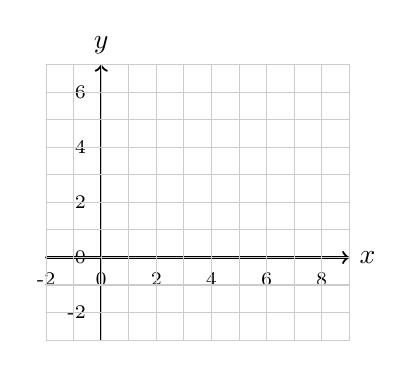
\begin{tikzpicture}[x=0.35cm, y=0.35cm, line cap=round, line join=round]
    \draw[thick,->] (-2,0) -- (9,0) node[right] {$x$};
    \draw[thick,->] (0,-3) -- (0,7) node[above] {$y$};
    \foreach \x in {-2,0,2,4,6,8} \draw (\x,2pt) -- (\x,-2pt) node[below,font=\scriptsize] {\x};
    \foreach \y in {-2,0,2,4,6} \draw (2pt,\y) -- (-2pt,\y) node[left,font=\scriptsize] {\y};
    \draw[gray!40] (-2,-3) grid[step=1] (9,7);
  \end{tikzpicture}
  \end{center}

  Domain: \blank[4em]

  Range: \blank[4em]

  Interval(s) of Increase: \blank[4em]

  Interval(s) of Decrease: \blank[4em]

  Concave Up: \blank[4em]

  Concave Down: \blank[4em]
  \vgapp


  \newpage
  \item Which of the following BEST describes the behavior of $g(x)$ over the interval $[-12,-4]$? \points{1}

  \begin{tasks}(1)
    \task Increasing with a decreasing rate of change
    \task Decreasing with an increasing rate of change
    \task Increasing with an increasing rate of change
    \task Decreasing with a decreasing rate of change
  \end{tasks}
  \vgap
  
  \item Solve the equation for $x$. Express all algebraic solutions. Then indicate any extraneous solutions. If there are no extraneous solutions, write ``no extraneous solutions.'' \points{4}
  \[
  4 - x = -2\sqrt{6-x}
  \]
  \vgappp


  \newpage
  \item Finish graphing $f(x)$ on the axes provided below. Then, identify the key features requested. All intervals MUST be expressed in interval notation (including concave up and concave down). \points{12}
  \[
  f(x)= \begin{cases}
    -(x-2)^{2}+5 & -2 \leq x<2 \\
    x+1 & 2<x<4 \\
    \sqrt{x-4}+1 & 4 \leq x<8 \\
    -\dfrac{x}{2}+5 & 8<x \leq 10
  \end{cases}
  \]

  \begin{center}
  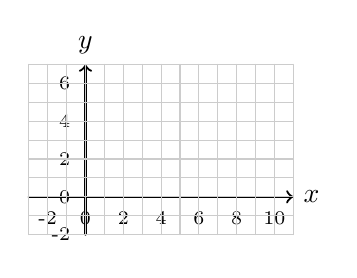
\begin{tikzpicture}[x=0.24cm, y=0.24cm, line cap=round, line join=round]
    \draw[thick,->] (-3,0) -- (11,0) node[right] {$x$};
    \draw[thick,->] (0,-2) -- (0,7) node[above] {$y$};
    \foreach \x in {-2,0,2,4,6,8,10} \draw (\x,2pt) -- (\x,-2pt) node[below,font=\scriptsize] {\x};
    \foreach \y in {-2,0,2,4,6} \draw (2pt,\y) -- (-2pt,\y) node[left,font=\scriptsize] {\y};
    \draw[gray!40] (-3,-2) grid[step=1] (11,7);
  \end{tikzpicture}
  \end{center}

  Domain: \blank

  Range: \blank

  Interval(s) of Increase: \blank

  Interval(s) of Decrease: \blank

  Concave Up: \blank

  Concave Down: \blank

  Absolute Minimum: \blank

  Absolute Maximum: \blank

  $\displaystyle \lim_{x \to 4^{-}} f(x) = $ \blank
  \vgapp


  \newpage
  \item Let $f(x)=\sqrt{x+3}$ and $g(x)=x^2-4$. Find the domain of $(f \circ g)(x)$ and write your answer in interval notation. \points{5}
  \vgappp

  \item Solve the inequality. Write your answer in interval notation.
  \[
  \sqrt{2x+5} \,-\, \sqrt{x-1} \;>\; 0
  \]
  \points{6}
  \vgappp

  \item The function $h(x)$ is obtained by reflecting the graph of $k(x)=\sqrt{9-x}$ across the $x$-axis, then shifting the result left by 2 units and up by 1 unit. (a) Write a formula for $h(x)$ in terms of $x$. (b) State the domain and range of $h(x)$ in interval notation. \points{6}
  \vgappp

\end{enumerate}
